\documentclass{article}

\usepackage[nonanonymous]{neurips_2026}
\makeatletter
\renewcommand{\@noticestring}{}
\makeatother

\usepackage[utf8]{inputenc}
\usepackage[T1]{fontenc}
\usepackage{graphicx}
\usepackage{hyperref}
\usepackage{url}
\usepackage{booktabs}
\usepackage{amsmath}
\usepackage{amsfonts}
\usepackage{nicefrac}
\usepackage{microtype}
\usepackage{xcolor}

\title{Making Self-Play Reinforcement Learning Feasible for Gomoku via Candidate Move Restriction}

\author{%
  Zengzheng Jiang \\
  \texttt{zengzheng@wustl.edu}
  \And
  En Wei \\
  \texttt{en@wustl.edu}
  \And
  Weizhi Du \\
  \texttt{d.weizhi@wustl.edu}
}


\begin{document}

\maketitle

\begin{abstract}
  AlphaZero-style self-play is conceptually appealing for Gomoku, but its practical cost grows quickly with board size because Monte Carlo Tree Search (MCTS) must repeatedly score a large number of legal moves at every position. This project studies whether a simple and interpretable candidate move restriction strategy can reduce that burden enough to make larger-board training feasible under limited compute. We implement an end-to-end Gomoku training pipeline with self-play, replay-buffer learning, a policy-value network, and both standard and pruning-aware MCTS. Our restriction rule keeps only legal moves inside a local window centered around the currently occupied region, and therefore shrinks the branching factor before node expansion. Experiments on several Gomoku settings show that the method preserves meaningful learning dynamics while substantially improving feasibility. In our reported runs, unrestricted training on an \(8 \times 8\) connect-5 setting required roughly 48 hours, whereas local restriction reduced that runtime to about 7 hours while still reaching a \(0.5\) final win ratio against pure MCTS; on an easier \(8 \times 8\) connect-4 setting, the pruned model achieved a final win ratio of \(1.0\) in roughly 3 hours. These results suggest that candidate move restriction is a practical first step toward scaling self-play reinforcement learning in board games with large discrete action spaces.
\end{abstract}

\section{Introduction}

Self-play reinforcement learning has become one of the most influential paradigms for game-playing AI because it removes the need for human demonstrations and allows a model to improve through repeated competition with itself. The AlphaGo Zero and AlphaZero lines of work showed that a policy-value network coupled with Monte Carlo Tree Search can achieve strong performance in games such as Go, chess, and shogi. However, these successes also highlight a practical limitation: the method is computationally expensive, and its cost rises sharply when the action space is large and most legal moves are strategically unimportant.

Gomoku is a good environment for studying this issue. The rules are simple, so implementation details do not dominate the project, but the search problem is still difficult. On larger boards, many available cells are obviously irrelevant because strong play usually concentrates near existing stones or urgent tactical threats. A naive self-play pipeline nevertheless treats every legal position as a candidate during MCTS expansion. As a result, a large amount of search effort is spent on moves that are unlikely to affect the game's outcome.

Our project asks a focused question: can an interpretable move restriction rule make AlphaZero-style self-play more feasible for Gomoku without destroying playing strength? We study this question by starting from a full AlphaZero-style baseline, then inserting a local candidate filter into both tree expansion and action selection. The resulting system still learns from self-play and still uses the policy network to guide search, but it explores only a restricted candidate set at each board state.

The project is motivated by two related goals. First, we want a practical training recipe for environments where the raw branching factor makes unrestricted self-play too slow. During development we found that moving from a \(6 \times 6\) board to an \(8 \times 8\) board already created a severe runtime increase, and a standard \(15 \times 15\) Gomoku board was beyond our available training budget. Second, we want the restriction mechanism to remain interpretable. Instead of introducing another large learned module only to decide which actions are worth evaluating, we prefer a rule that can be reasoned about directly and adjusted with minimal engineering effort.

The main contributions of this report are:
\begin{itemize}
  \item We implement a complete AlphaZero-style Gomoku pipeline with self-play, data augmentation, replay-buffer learning, evaluation against external opponents, and training metric logging.
  \item We introduce a candidate move restriction mechanism based on a local search window around existing stones, and integrate it directly into the MCTS procedure.
  \item We evaluate the method on multiple board/rule settings and show that pruning substantially improves runtime feasibility while preserving useful learning behavior, although the hardest setting still exhibits a clear efficiency-strength trade-off.
  \item We use these results to discuss when simple action-space restriction is helpful, what biases it introduces, and how the method could be extended with threat-aware or policy-guided filters in future work.
\end{itemize}

Overall, the central claim of this report is not that local-window pruning solves Gomoku completely. Rather, it provides a simple, effective, and computationally affordable way to make self-play reinforcement learning on larger Gomoku boards much more practical.

\section{Related Work}

This work is most directly connected to AlphaGo Zero and AlphaZero, which combine neural policy-value prediction with MCTS and self-play training [1, 2]. Those systems demonstrated that strong performance can emerge from repeated self-play without human policy supervision, but they also required substantial computation. Their success motivates our baseline design, while their computational demands motivate our search for a more efficient action-selection mechanism.

Our project also builds on the broader MCTS literature. Bandit-based tree search methods such as UCT formalized the balance between exploration and exploitation in sequential decision problems [3], and later surveys documented many ways to improve MCTS efficiency in practice [4]. In board games, pruning or heuristic move ordering is often used to reduce wasted search. Our approach fits naturally into this tradition: we do not replace MCTS, but instead constrain the legal actions it expands at each node.

Several works are especially relevant for Gomoku. Liang et al.\ study an AlphaZero-style system for Gomoku and show that the framework can learn effective policies for the game [5]. Their work supports the premise that AlphaZero is a sensible baseline for Gomoku, but their focus is not on reducing search cost via explicit candidate restriction. Fujita's AlphaViT explores a flexible game-playing framework across different board games and board sizes [6], highlighting how model performance and computational requirements interact with environment scale. That perspective aligns with our observation that the board-size increase from \(6 \times 6\) to \(8 \times 8\) substantially changes feasibility, not just final performance.

The gap we address is therefore narrower and more practical than the gaps addressed in those prior papers. We are not primarily trying to show that AlphaZero works for Gomoku, nor are we designing a new network architecture. Instead, we ask whether a simple, interpretable restriction on the action space can make self-play training on larger Gomoku boards feasible under limited resources. This question is relevant beyond Gomoku because many reinforcement learning problems with large discrete action spaces face the same issue: most actions are legal, but only a small subset are worth careful search.

Finally, our work relates to the general idea of injecting domain knowledge into learning systems. Classical board-game programs often rely on tactical patterns, local neighborhoods, and handcrafted move ordering. AlphaZero-style methods deliberately reduce such prior assumptions, but in resource-constrained settings, mild structural bias can be valuable. Our local-window rule is a particularly lightweight form of domain knowledge: it assumes that informative moves tend to occur near existing stones, yet it remains easy to implement, inspect, and refine. The method is therefore best understood as a practical bridge between unconstrained end-to-end self-play and more heavily engineered search heuristics.

\section{Background \& Preliminaries}

In Gomoku, two players alternate placing stones on a rectangular grid, and the first player to form a line of \(n\) consecutive stones horizontally, vertically, or diagonally wins. Our experiments use several rule settings, including \(6 \times 6\) connect-4 and \(8 \times 8\) boards with either connect-4 or connect-5 winning conditions. At each state \(s\), the legal action space \(A(s)\) is the set of currently empty cells.

The baseline learning pipeline follows the AlphaZero pattern. A self-play game is generated by repeatedly calling an MCTS-based player. For each visited state, the system stores the board representation, the search policy returned by MCTS, and the final game outcome. These transitions are then augmented by board symmetries, added to a replay buffer, and used to update a neural policy-value network.

Our implementation uses a four-plane board encoding. Given the current player's perspective, the first plane marks the current player's stones, the second plane marks the opponent's stones, the third plane marks the previous move, and the fourth plane indicates whose turn it is. This encoding is passed through a convolutional network with a shared trunk and two heads: a policy head that predicts move probabilities over the board, and a value head that predicts the expected outcome of the current position.

Within MCTS, each tree node stores a prior \(P\), visit count \(N\), and running action value \(Q\). Child selection follows the usual AlphaZero-style upper-confidence rule
\begin{equation}
  a^\star = \arg\max_a \left( Q(s,a) + U(s,a) \right), \quad
  U(s,a) = c_{\text{puct}} P(s,a)\frac{\sqrt{\sum_b N(s,b)}}{1 + N(s,a)}.
\end{equation}
After descending to a leaf, the policy-value network returns a set of move priors together with a scalar leaf value in \([-1,1]\). The priors are used to expand new child nodes, and the value is backed up through the search path.

Training optimizes the standard joint policy-value objective
\begin{equation}
  \mathcal{L} = (z - v)^2 - \pi^\top \log p + \lambda \lVert \theta \rVert_2^2,
\end{equation}
where \(z\) is the game outcome, \(v\) is the predicted state value, \(\pi\) is the MCTS-improved target policy, and \(p\) is the network's policy output. In practice, our code also monitors KL divergence between successive policy outputs and adaptively rescales the learning rate multiplier when updates become too large or too small.

The key computational issue is that MCTS expansion must handle all legal moves returned by the network. If the board is large, the branching factor quickly becomes expensive even when most moves are strategically weak. This motivates the central object of our report: a candidate set \(C(s) \subseteq A(s)\) that removes obviously unhelpful moves before search expansion.

\section{Method}

Our method starts from a standard AlphaZero-style Gomoku pipeline and modifies only one part of the decision process: the set of actions expanded by MCTS. This choice is intentional. By holding the rest of the pipeline fixed, we can attribute changes in runtime and performance primarily to candidate move restriction rather than to unrelated architectural changes.

\subsection{Baseline pipeline}

The baseline system contains four core components. First, the game engine maintains the board state, legal moves, and win detection. Second, the policy-value network maps the four-plane board representation to a move distribution and a scalar value. Third, the MCTS module uses the network to guide selection and expansion. Fourth, the training loop orchestrates self-play, replay-buffer storage, minibatch updates, periodic evaluation, and model checkpointing.

For each self-play game, the current MCTS player generates move probabilities. The resulting trajectory is then augmented by rotation and reflection, which effectively multiplies the amount of supervised signal obtained from each finished game. Once the replay buffer is sufficiently populated, the system samples minibatches and performs several epochs of gradient updates. Every fixed number of batches, the current model is evaluated against either a pure MCTS opponent or a stronger pretrained model, depending on the experiment.

\subsection{Local candidate move restriction}

The proposed pruning rule is deliberately simple. Given a board state, we compute the centroid of all currently occupied cells and place a fixed-size local window around that center. On an \(8 \times 8\) board, our current implementation uses a \(6 \times 6\) window. The candidate set \(C(s)\) is then defined as the legal moves that fall inside this window:
\begin{equation}
  C(s) = \{ a \in A(s) \mid a \text{ lies inside the centered local window} \}.
\end{equation}
If the board is already smaller than the window, or if the filtered set is accidentally empty, the implementation falls back to the full legal move list. This safeguard keeps the procedure robust and prevents pathological failures.

This rule captures a basic empirical property of Gomoku: meaningful moves usually cluster around the active region of the board. Early in the game, when few stones have been placed, the full board or nearly full board remains available. As the game develops, however, the restriction cuts away remote cells that are unlikely to matter immediately. Because the window is computed from the state itself, the rule is adaptive even though its window size is fixed.

\subsection{Where pruning enters MCTS}

We integrate pruning in two places. During a playout, after the policy-value network returns action priors, we filter those priors so that only moves in \(C(s)\) are expanded as children. The filtered probabilities are then renormalized before node expansion. During action selection at the root, the player also limits the sensible move set to the same pruned candidate set. This ensures consistency between what the search explores and what the agent is willing to choose.

Conceptually, the difference from standard MCTS is:
\begin{equation}
  \text{standard expansion: } \mathrm{Expand}(A(s)), \qquad
  \text{pruned expansion: } \mathrm{Expand}(C(s)).
\end{equation}
The computational benefit comes from reducing the number of children considered at each node, which in turn shrinks the effective search tree. The cost is that the search may miss tactically important remote moves if the local-window assumption fails.

\subsection{Expected benefits and biases}

The expected benefit of pruning is straightforward: with fewer candidate moves, each playout spends less effort on low-value branches, so the same hardware budget can cover more training batches or larger boards. This is especially important in our environment because MCTS is the dominant computational bottleneck. Unlike the neural network updates, tree search does not benefit as much from GPU parallelism in our implementation, so reducing the branching factor directly saves wall-clock time.

At the same time, pruning introduces bias. It assumes that good moves remain local to the current stone distribution. While this is often true in Gomoku, it is not universally true, especially in tactical positions where long-range blocking or setup moves matter. Because of this trade-off, we treat pruning as a feasibility-oriented approximation rather than a guarantee of optimal play.

\subsection{Planned extensions}

The current local-window rule is only the first version of the broader idea. During the project we also considered several extensions: threat-aware exceptions that force the candidate set to include urgent attack or defense moves, policy top-\(k\) filtering based on the network's own prior distribution, and simple heuristic scores that rank legal cells by local pattern quality. These variants are not yet supported by the same level of empirical evidence as the local-window rule, so we do not present them as finished contributions. Nevertheless, they clarify the long-term direction of the project: local restriction is useful, but combining locality with tactical awareness is likely the most promising path forward.

\section{Experiments}

We evaluate whether candidate move restriction makes self-play training more feasible while preserving useful performance. All experiments are conducted in our own AlphaZero-style Gomoku codebase. The main training hyperparameters are consistent across runs unless the game setting itself changes: learning rate \(2\times10^{-3}\), \(c_{\text{puct}}=5\), 400 playouts for the neural MCTS player, replay buffer size 10{,}000, batch size 512, 5 training epochs per update, evaluation every 50 batches, and 1{,}500 self-play batches per full run. Data are generated entirely by self-play and augmented with rotations and reflections before being inserted into the replay buffer.

\subsection{Experimental settings}

We focus on four representative settings:
\begin{enumerate}
  \item an unrestricted \(6 \times 6\) connect-4 baseline,
  \item a pruned \(8 \times 8\) connect-4 model evaluated against pure MCTS,
  \item a pruned \(8 \times 8\) connect-5 model evaluated against pure MCTS, and
  \item a pruned \(8 \times 8\) connect-5 model evaluated against a pretrained \(8 \times 8\) connect-5 policy.
\end{enumerate}

The unrestricted \(8 \times 8\) connect-5 baseline is also important conceptually, even though it is too expensive to serve as our main fully evaluated comparison. According to our project logs and presentation materials, that setting required roughly 48 hours of training, which made repeated experimentation impractical. This runtime bottleneck is exactly the problem that motivated pruning.

We monitor several metrics throughout training: self-play episode length, replay buffer size, training loss, policy entropy, effective learning rate, and evaluation win ratio. The win ratio is the most direct summary of playing strength in our experiments, while loss and entropy help show whether the model is learning structured behavior instead of merely saving time by training less.

\subsection{Main quantitative results}

Table~\ref{tab:main-results} summarizes the most important outcomes used in the report. Runtime values are the reported wall-clock times from our project materials, while final/best win ratios come from the saved training summaries. The table should be interpreted carefully: results are directly comparable only when the evaluation opponent is the same.

\begin{table}[t]
  \caption{Summary of representative training runs. Reported runtimes come from our project records and slides; final/best win ratios come from the saved run summaries.}
  \label{tab:main-results}
  \centering
  \begin{tabular}{lllll}
    \toprule
    Setting & Restriction & Eval opponent & Runtime & Final / best win ratio \\
    \midrule
    \(6 \times 6\), connect-4 & none & pure MCTS & \(\sim\)3h & 0.90 / 0.90 \\
    \(8 \times 8\), connect-5 & none & not completed & \(\sim\)48h & N/A \\
    \(8 \times 8\), connect-4 & local \(6 \times 6\) window & pure MCTS & \(\sim\)3h & 1.00 / 1.00 \\
    \(8 \times 8\), connect-5 & local \(6 \times 6\) window & pure MCTS & \(\sim\)7h & 0.50 / 0.60 \\
    \(8 \times 8\), connect-5 & local \(6 \times 6\) window & pretrained \(8 \times 8\) & not logged & 0.00 / 0.00 \\
    \bottomrule
  \end{tabular}
\end{table}

The strongest headline result is the runtime change on the hardest setting we could partially compare. Moving from the unrestricted \(8 \times 8\) connect-5 baseline to the pruned version reduces the reported training time from about 48 hours to about 7 hours, a reduction of roughly \(6.9\times\). This is a substantial practical gain: it changes the experiment from something that is difficult to iterate on into something that can realistically be rerun and tuned within a course project.

On the easier \(8 \times 8\) connect-4 setting, pruning appears especially effective. The pruned model reaches a final and best win ratio of \(1.0\) against pure MCTS while staying in the same rough runtime regime as the much smaller \(6 \times 6\) baseline. This suggests that candidate restriction is not merely saving time by weakening the problem; instead, on moderate settings it can preserve or even improve effective learning progress by concentrating search on more relevant actions.

The \(8 \times 8\) connect-5 setting is more revealing about the method's limits. Against pure MCTS, the pruned model still reaches a final win ratio of \(0.5\) and a best recorded win ratio of \(0.6\), which indicates competitive but not dominant strength. Against a stronger pretrained \(8 \times 8\) connect-5 model, however, the same local restriction is not sufficient: the final and best win ratios remain at \(0.0\). This result is consistent with the intuition that pruning helps feasibility first, but can discard tactically important moves when the task becomes sufficiently demanding.

\subsection{Training dynamics}

The logged metrics also support the claim that pruning produces real learning rather than superficial speedups. Figure~\ref{fig:loss} shows that the training loss decreases over time in the representative runs, although the harder \(8 \times 8\) connect-5 setting remains at a higher loss level than the \(6 \times 6\) baseline and the pruned \(8 \times 8\) connect-4 configuration. This is exactly what we would expect if the larger board and harder win condition create a more difficult optimization problem.

\begin{figure}[t]
  \centering
  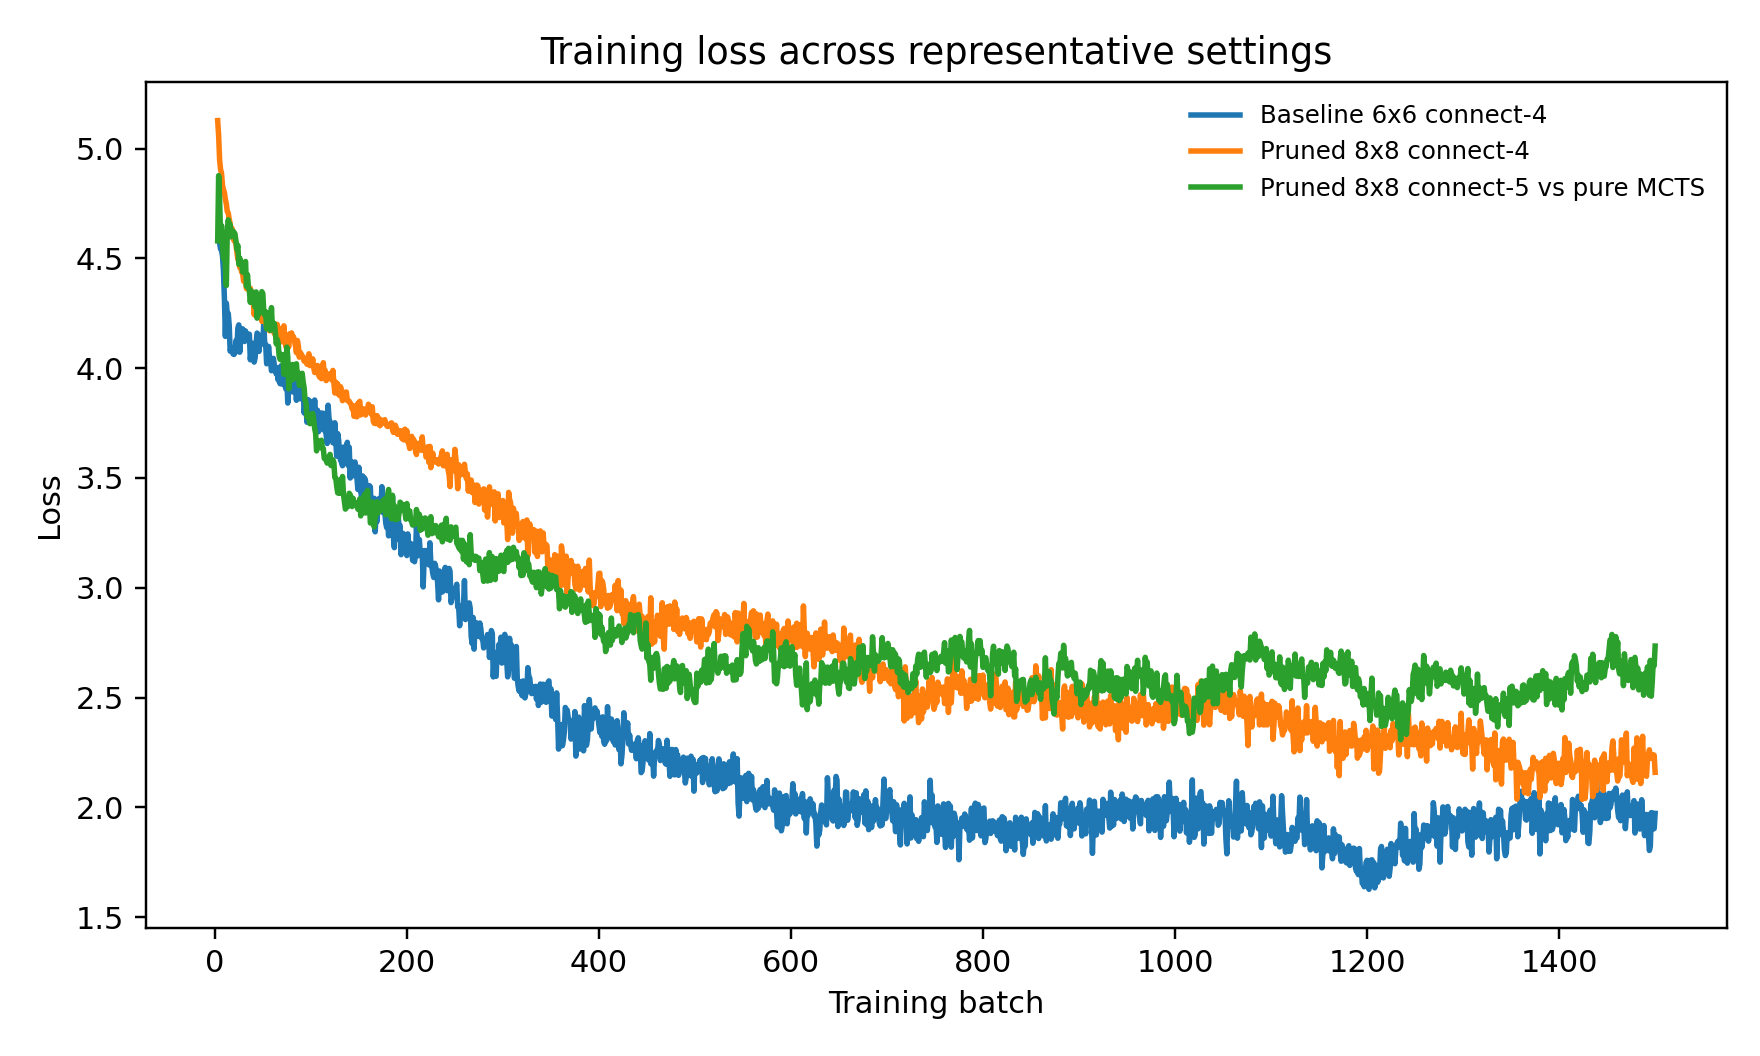
\includegraphics[width=0.95\linewidth]{plots/loss_comparison.png}
  \caption{Training loss across representative settings. The harder \(8 \times 8\) connect-5 run remains more difficult to optimize than the \(6 \times 6\) baseline and the pruned \(8 \times 8\) connect-4 setting, but all runs still exhibit meaningful training dynamics rather than degenerate behavior.}
  \label{fig:loss}
\end{figure}

Policy entropy shows a similar pattern. In our saved summaries, the final entropy values are approximately 1.36 for the \(6 \times 6\) baseline, 1.53 for pruned \(8 \times 8\) connect-4, and 1.95 for pruned \(8 \times 8\) connect-5 against pure MCTS. Lower entropy here indicates that the policy is becoming more decisive. The fact that the harder setting remains more entropic supports the claim that the task is genuinely more uncertain, not that the system is failing to train altogether.

Episode length is also informative. The final self-play episode lengths are 15 for the unrestricted \(6 \times 6\) baseline, 12 for pruned \(8 \times 8\) connect-4, and 14 for pruned \(8 \times 8\) connect-5 against pure MCTS. These values indicate that pruning does not simply collapse games immediately; instead, the training loop continues to generate full sequences of moves with plausible game lengths, which are then used to update the model.

Figure~\ref{fig:winratio} presents the evaluation win ratio trajectories. Two observations stand out. First, the pruned \(8 \times 8\) connect-4 run is consistently strong, which makes it a convincing proof of concept for the pruning idea. Second, the gap between the pruned \(8 \times 8\) connect-5 runs against different opponents illustrates that evaluation context matters. A win ratio against pure MCTS should not be interpreted as equivalent to the same number against a much stronger pretrained policy.

\begin{figure}[t]
  \centering
  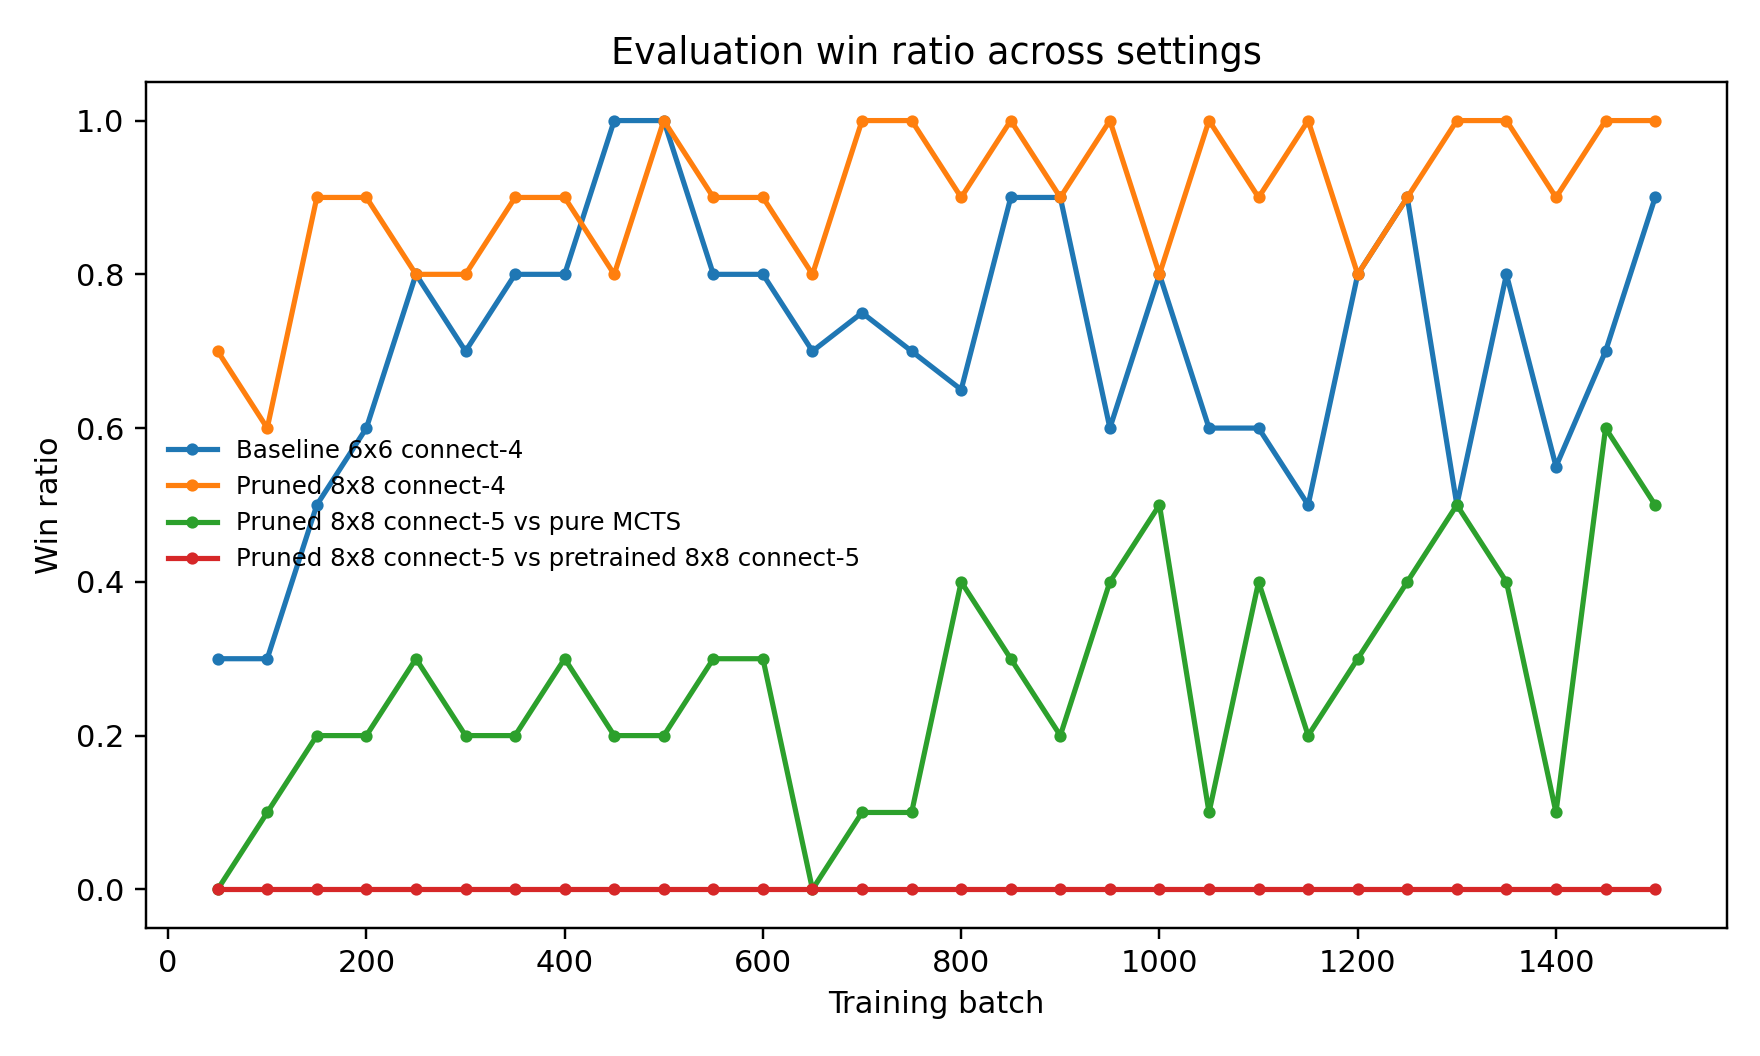
\includegraphics[width=0.95\linewidth]{plots/win_ratio_comparison.png}
  \caption{Evaluation win ratio across settings. Local pruning remains competitive on \(8 \times 8\) connect-5 against pure MCTS and performs very well on \(8 \times 8\) connect-4, but it does not yet recover enough strength to beat a stronger pretrained \(8 \times 8\) connect-5 opponent.}
  \label{fig:winratio}
\end{figure}

\subsection{Ablation-style interpretation}

Although our experimental matrix is not exhaustive, the available results still support an ablation-style interpretation. The main variable being changed between the standard and pruned search pipelines is whether MCTS expands the full legal set or a local candidate subset. Because the rest of the training pipeline stays largely unchanged, the large runtime difference on \(8 \times 8\) connect-5 is strong evidence that candidate restriction is the central source of the feasibility gain.

At the same time, the results show that pruning strength depends on task difficulty. On easier settings, the local-window assumption is strong enough that removing remote moves does not appear harmful. On the hardest setting, however, the same rule likely over-prunes. This suggests that candidate restriction is valuable not as a universal replacement for unrestricted search, but as a tunable approximation whose aggressiveness should depend on board size, win condition, and opponent strength.

\subsection{Discussion}

Taken together, the experiments support three conclusions. First, our AlphaZero-style Gomoku implementation is working end to end: losses decrease, entropy changes, replay buffers fill, and evaluation scores improve in several settings. Second, candidate move restriction addresses the bottleneck we actually observed in practice, namely the cost of MCTS on larger boards. Third, the method introduces a real trade-off. It is highly useful for feasibility, but the strongest setting in our study indicates that simple locality alone is not enough to preserve full strength.

This trade-off is still a positive result. In a course-project setting with limited hardware, reducing a 48-hour run to about 7 hours is not just a marginal improvement. It fundamentally changes which experiments are possible. Even when pruning does not preserve all of the original search strength, it makes iteration, debugging, and hyperparameter exploration much more realistic.

\section{Conclusions}

This project studies whether self-play reinforcement learning for Gomoku can be made more practical by reducing the effective action space seen by MCTS. Starting from an AlphaZero-style baseline, we introduced a simple local candidate move restriction rule and integrated it into the search procedure without changing the rest of the learning pipeline.

The results show that this idea is useful. The pruning-based system preserves meaningful learning dynamics, performs strongly on moderate settings such as \(8 \times 8\) connect-4, and greatly improves feasibility on harder settings by reducing runtime. The clearest example is the shift from an approximately 48-hour unrestricted \(8 \times 8\) connect-5 run to an approximately 7-hour pruned run. At the same time, the method does not fully preserve strength on the hardest evaluations, which means the local-window restriction should be viewed as a practical approximation rather than a complete solution.

Overall, our findings support the central hypothesis of the project: candidate move restriction can make self-play reinforcement learning for Gomoku substantially more feasible under limited computational resources, and it provides a promising foundation for stronger, more adaptive pruning methods.

\section{Limitations \& Future Work}

The most important limitation of the current project is that our pruning rule is intentionally simple. A fixed local window is easy to interpret and fast to compute, but it can exclude tactically critical moves that lie outside the active region estimated by the centroid of existing stones. This is the most likely explanation for the weaker results on the hardest \(8 \times 8\) connect-5 evaluations.

Another limitation is that our experimental comparisons are not fully symmetric. Some runs are evaluated against pure MCTS, while one of the hardest settings is evaluated against a stronger pretrained \(8 \times 8\) connect-5 policy. This is still useful for understanding the method's ceiling, but it means that win ratios across all rows should not be compared as if they came from the same benchmark. In addition, the unrestricted \(8 \times 8\) connect-5 baseline was expensive enough that we could not build as complete an evaluation record for it as we did for the smaller or pruned settings.

There are also implementation-level limitations. The current code hard-codes the pruning window size, so the system cannot yet adapt restriction strength dynamically over training or across board states. Our network architecture is intentionally modest, which is appropriate for a course project but may underrepresent what a stronger policy-value network could achieve with the same pruning rule. Finally, the project focuses only on Gomoku, so the generality of the approach to other large-action-space domains remains a hypothesis rather than an empirical claim.

These limitations suggest several concrete directions for future work. The first is threat-aware pruning: local windows could be supplemented with pattern detectors that always include moves creating or blocking open threes, open fours, and similar tactical motifs. The second is policy-guided filtering, where the candidate set combines a local rule with the top-\(k\) moves from the policy network. The third is adaptive pruning strength, in which the system uses stronger restriction early in training or in quiet positions and weaker restriction in tactically sharp positions. A final extension would be to test the same idea in other domains with large discrete action spaces, such as other board games or simplified robotic planning tasks.

In short, the current report demonstrates that interpretable candidate restriction is already useful, but it also makes clear that the best long-term version of the idea will likely combine locality, tactical awareness, and learned guidance rather than relying on any single heuristic alone.

\section*{References}

{\small

[1] Silver, D., Schrittwieser, J., Simonyan, K., Antonoglou, I., Huang, A., Guez, A., Hubert, T., Baker, L., Lai, M., Bolton, A., et al.\ (2017) Mastering the game of Go without human knowledge. {\it Nature} {\bf 550}(7676):354--359.

[2] Silver, D., Hubert, T., Schrittwieser, J., Antonoglou, I., Lai, M., Guez, A., Lanctot, M., Sifre, L., Kumaran, D., Graepel, T., Lillicrap, T., Simonyan, K.\ \& Hassabis, D.\ (2018) A general reinforcement learning algorithm that masters chess, shogi, and Go through self-play. {\it Science} {\bf 362}(6419):1140--1144.

[3] Kocsis, L.\ \& Szepesv\'ari, C.\ (2006) Bandit based Monte-Carlo planning. In {\it Proceedings of the 17th European Conference on Machine Learning}, pp.\ 282--293.

[4] Browne, C.B., Powley, E., Whitehouse, D., Lucas, S., Cowling, P.I., Rohlfshagen, P., Tavener, S., Perez, D., Samothrakis, S.\ \& Colton, S.\ (2012) A survey of Monte Carlo tree search methods. {\it IEEE Transactions on Computational Intelligence and AI in Games} {\bf 4}(1):1--43.

[5] Liang, W., Yu, C., Whiteaker, B., Huh, I., Shao, H.\ \& Liang, Y.\ (2023) AlphaZero Gomoku. {\it arXiv preprint arXiv:2309.01294}.

[6] Fujita, K.\ (2025) AlphaViT: A flexible game-playing AI for multiple games and variable board sizes. {\it PeerJ Computer Science} {\bf 11}:e3403.
}

\end{document}
